% !TEX root = ../lab1_report.tex
% ==========================================================
% 实验一：发动机模拟试车实验
% ==========================================================
\section{实验一：发动机模拟试车实验}

\subsection{实验目的}

\begin{enumerate}
    \item 通过本实验使学生了解发动机特性的实验方法和实验过程，掌握发动机主要性能参数的测量和数据处理方法，同时进一步加深学生对发动机特性知识的认识。
    \item 确定下列发动机特性曲线：
    \begin{itemize}
        \item \textbf{节流特性曲线（必做）}
        \begin{align*}
            F &= f(n_{1}) & \alpha_1 &= f(n_{1}) \\
            \pi_c^* &= f(n_{2}) & \alpha_2 &= f(n_{2}) \\
            F &= f(n_{2}) & \text{sfc} &= f(n_{2}) \\
            m_a &= f(n_{2})
        \end{align*}
        \item \textbf{加力特性曲线（选做）}
        \begin{align*}
            F_{af} &= f(\text{油门杆位置}) \\
            \text{sfc}_{af} &= f(\text{油门杆位置}) \\
            A_e &= f(\text{油门杆位置})
        \end{align*}
    \end{itemize}
    \item 能力培养：实际试验操作能力、团结协作能力、综合应用能力。
\end{enumerate}

\subsection{实验设备简介}

该实验装置是一套发动机模拟试车系统，根据发动机地面台架试车台的功能进行模拟仿真，试车操作界面与实际发动机试车台基本相同。系统由油门杆、控制操作面板和计算机系统组成。

进行模拟试车的目的一方面为了取得发动机特性的具体试验数据，另一方面也为学生今后进行真实发动机开车试验积累实践经验，因此学生必须像对待真实发动机试车那样严肃认真。

主要测量参数：
\begin{itemize}
    \item 大气参数：$P_0$（大气压力）、$T_0$（大气温度）
    \item 性能参数：$F$（推力）、$W_f$（燃油消耗量）、$m_a$（空气流量）
    \item 转子参数：$n_1$（低压转子转速）、$n_2$（高压转子转速）
    \item 截面参数：$P_2^*$、$T_2^*$（风扇出口）、$P_3^*$、$T_3^*$（压气机出口）、$P_5^*$、$T_5^*$（涡轮后）
    \item 控制参数：$\alpha_1$、$\alpha_2$（导流叶片角度）、$A_t$（喷口喉道面积）
\end{itemize}

\subsection{数据记录列表}

实验数据按附表1格式记录，包含慢车状态至加力状态共13个工作状态的完整参数。

% \begin{table}[H]
%   \centering
%   \caption{发动机模拟试车实验数据}
%   \label{tab:exp1_trial}
%   \footnotesize
%   \setlength{\tabcolsep}{3pt}
%   \begin{tabular}{cccccccccc}
%     \toprule
%     工作状态 & $n_1$ & $n_2$ & $F$(N) & $W_f$(kg/h) & $m_a$(kg/s) & $\pi_c^*$ & sfc(h$^{-1}$) & $\alpha_1$ & $\alpha_2$ \\
%     \midrule
%     慢车 & 72.5 & 32.9 & 3424 & 461 & 40.4 & 4.09 & 1.3195 & 7 & 5 \\
%     N2=75% & 75.5 & 33.8 & 6317 & 656 & 47.4 & 4.32 & 1.0183 & 7 & 6 \\
%     N2=80% & 80.3 & 40.0 & 17889 & 1429 & 59.5 & 4.73 & 0.7837 & 7 & 39 \\
%     N2=85% & 85.1 & 60.1 & 29148 & 2057 & 70.9 & 5.25 & 0.6924 & 7 & 75 \\
%     N2=90% & 90.2 & 82.4 & 41312 & 2898 & 81.5 & 5.70 & 0.6882 & 16 & 105 \\
%     N2=95% & 95.3 & 92.0 & 54391 & 3922 & 92.7 & 6.09 & 0.7074 & 85 & 105 \\
%     N2=97% & 97.1 & 94.5 & 59141 & 4346 & 96.3 & 6.21 & 0.7209 & 97 & 105 \\
%     最大 & 99.9 & 97.9 & 66177 & 5027 & 100.7 & 6.41 & 0.7452 & 105 & 105 \\
%     加力_a=0 & 83.2 & 97.9 & 79311 & 8182 & 100.8 & 6.41 & 1.0120 & 105 & 105 \\
%     加力_a=1 & 88.8 & 97.9 & 83930 & 9820 & 100.7 & 6.41 & 1.1478 & 105 & 105 \\
%     加力_a=2 & 99.6 & 97.9 & 94227 & 14103 & 100.7 & 6.41 & 1.4682 & 105 & 105 \\
%     加力_a=3 & 108.0 & 97.9 & 104091 & 18408 & 100.7 & 6.41 & 1.7349 & 105 & 105 \\
%     加力_a=4 & 114.7 & 97.9 & 113465 & 22462 & 100.7 & 6.41 & 1.9420 & 105 & 105 \\
%     \bottomrule
%   \end{tabular}
% \end{table}

\begin{tabular}{|c|*{15}{c|}} % 第1列自适应宽度，后15列采用自定义的固定宽度 C
    \hline
    % 使用 \diagbox 绘制斜线表头，并配合 \makecell 换行
    \diagbox[width=3.6cm, height=1.3cm]{工作状态}{\makecell{参数名称 \\ (单位)}} & 
    $n_1$ & $P_0$ & $T_0$ & $F$ & $W_f$ & $m_a$ & $P_2^*$ & $T_2^*$ & $P_3^*$ & $T_3^*$ & $P_5^*$ & $T_5^*$ & $\alpha_1$ & $\alpha_2$ & $A_t$ \\
    \hline
    \makecell{慢车状态 \\ (N2=\hspace{1cm})} & & & & & & & & & & & & & & & \\
    \hline
    N2=75\% & & & & & & & & & & & & & & & \\
    \hline
    N2=80\% & & & & & & & & & & & & & & & \\
    \hline
    N2=85\% & & & & & & & & & & & & & & & \\
    \hline
    N2=90\% & & & & & & & & & & & & & & & \\
    \hline
    N2=95\% & & & & & & & & & & & & & & & \\
    \hline
    N2=97\% & & & & & & & & & & & & & & & \\
    \hline
    \makecell{最大状态 \\ (N2=\hspace{1cm})} & & & & & & & & & & & & & & & \\
    \hline
    \makecell{加力状态 \\ ($a_0$=\hspace{1cm})} & & & & & & & & & & & & & & & \\
    \hline
    \makecell{加力状态 \\ ($a_0$=\hspace{1cm})} & & & & & & & & & & & & & & & \\
    \hline
    \makecell{加力状态 \\ ($a_0$=\hspace{1cm})} & & & & & & & & & & & & & & & \\
    \hline
    \makecell{加力状态 \\ ($a_0$=\hspace{1cm})} & & & & & & & & & & & & & & & \\
    \hline
    \makecell{加力状态 \\ ($a_0$=\hspace{1cm})} & & & & & & & & & & & & & & & \\
    \hline
\end{tabular}

\subsection{数据处理方法}

\subsubsection{耗油率计算}

\begin{equation}
    \text{sfc} = \frac{W_f}{F}
\end{equation}

\subsubsection{压气机总压比}

\begin{equation}
    \pi_c^* = \frac{P_3^*}{P_2^*}
\end{equation}

\subsection{数据处理结果（曲线）及分析}

\subsubsection{节流特性曲线}

\begin{figure}[H]
    \centering
    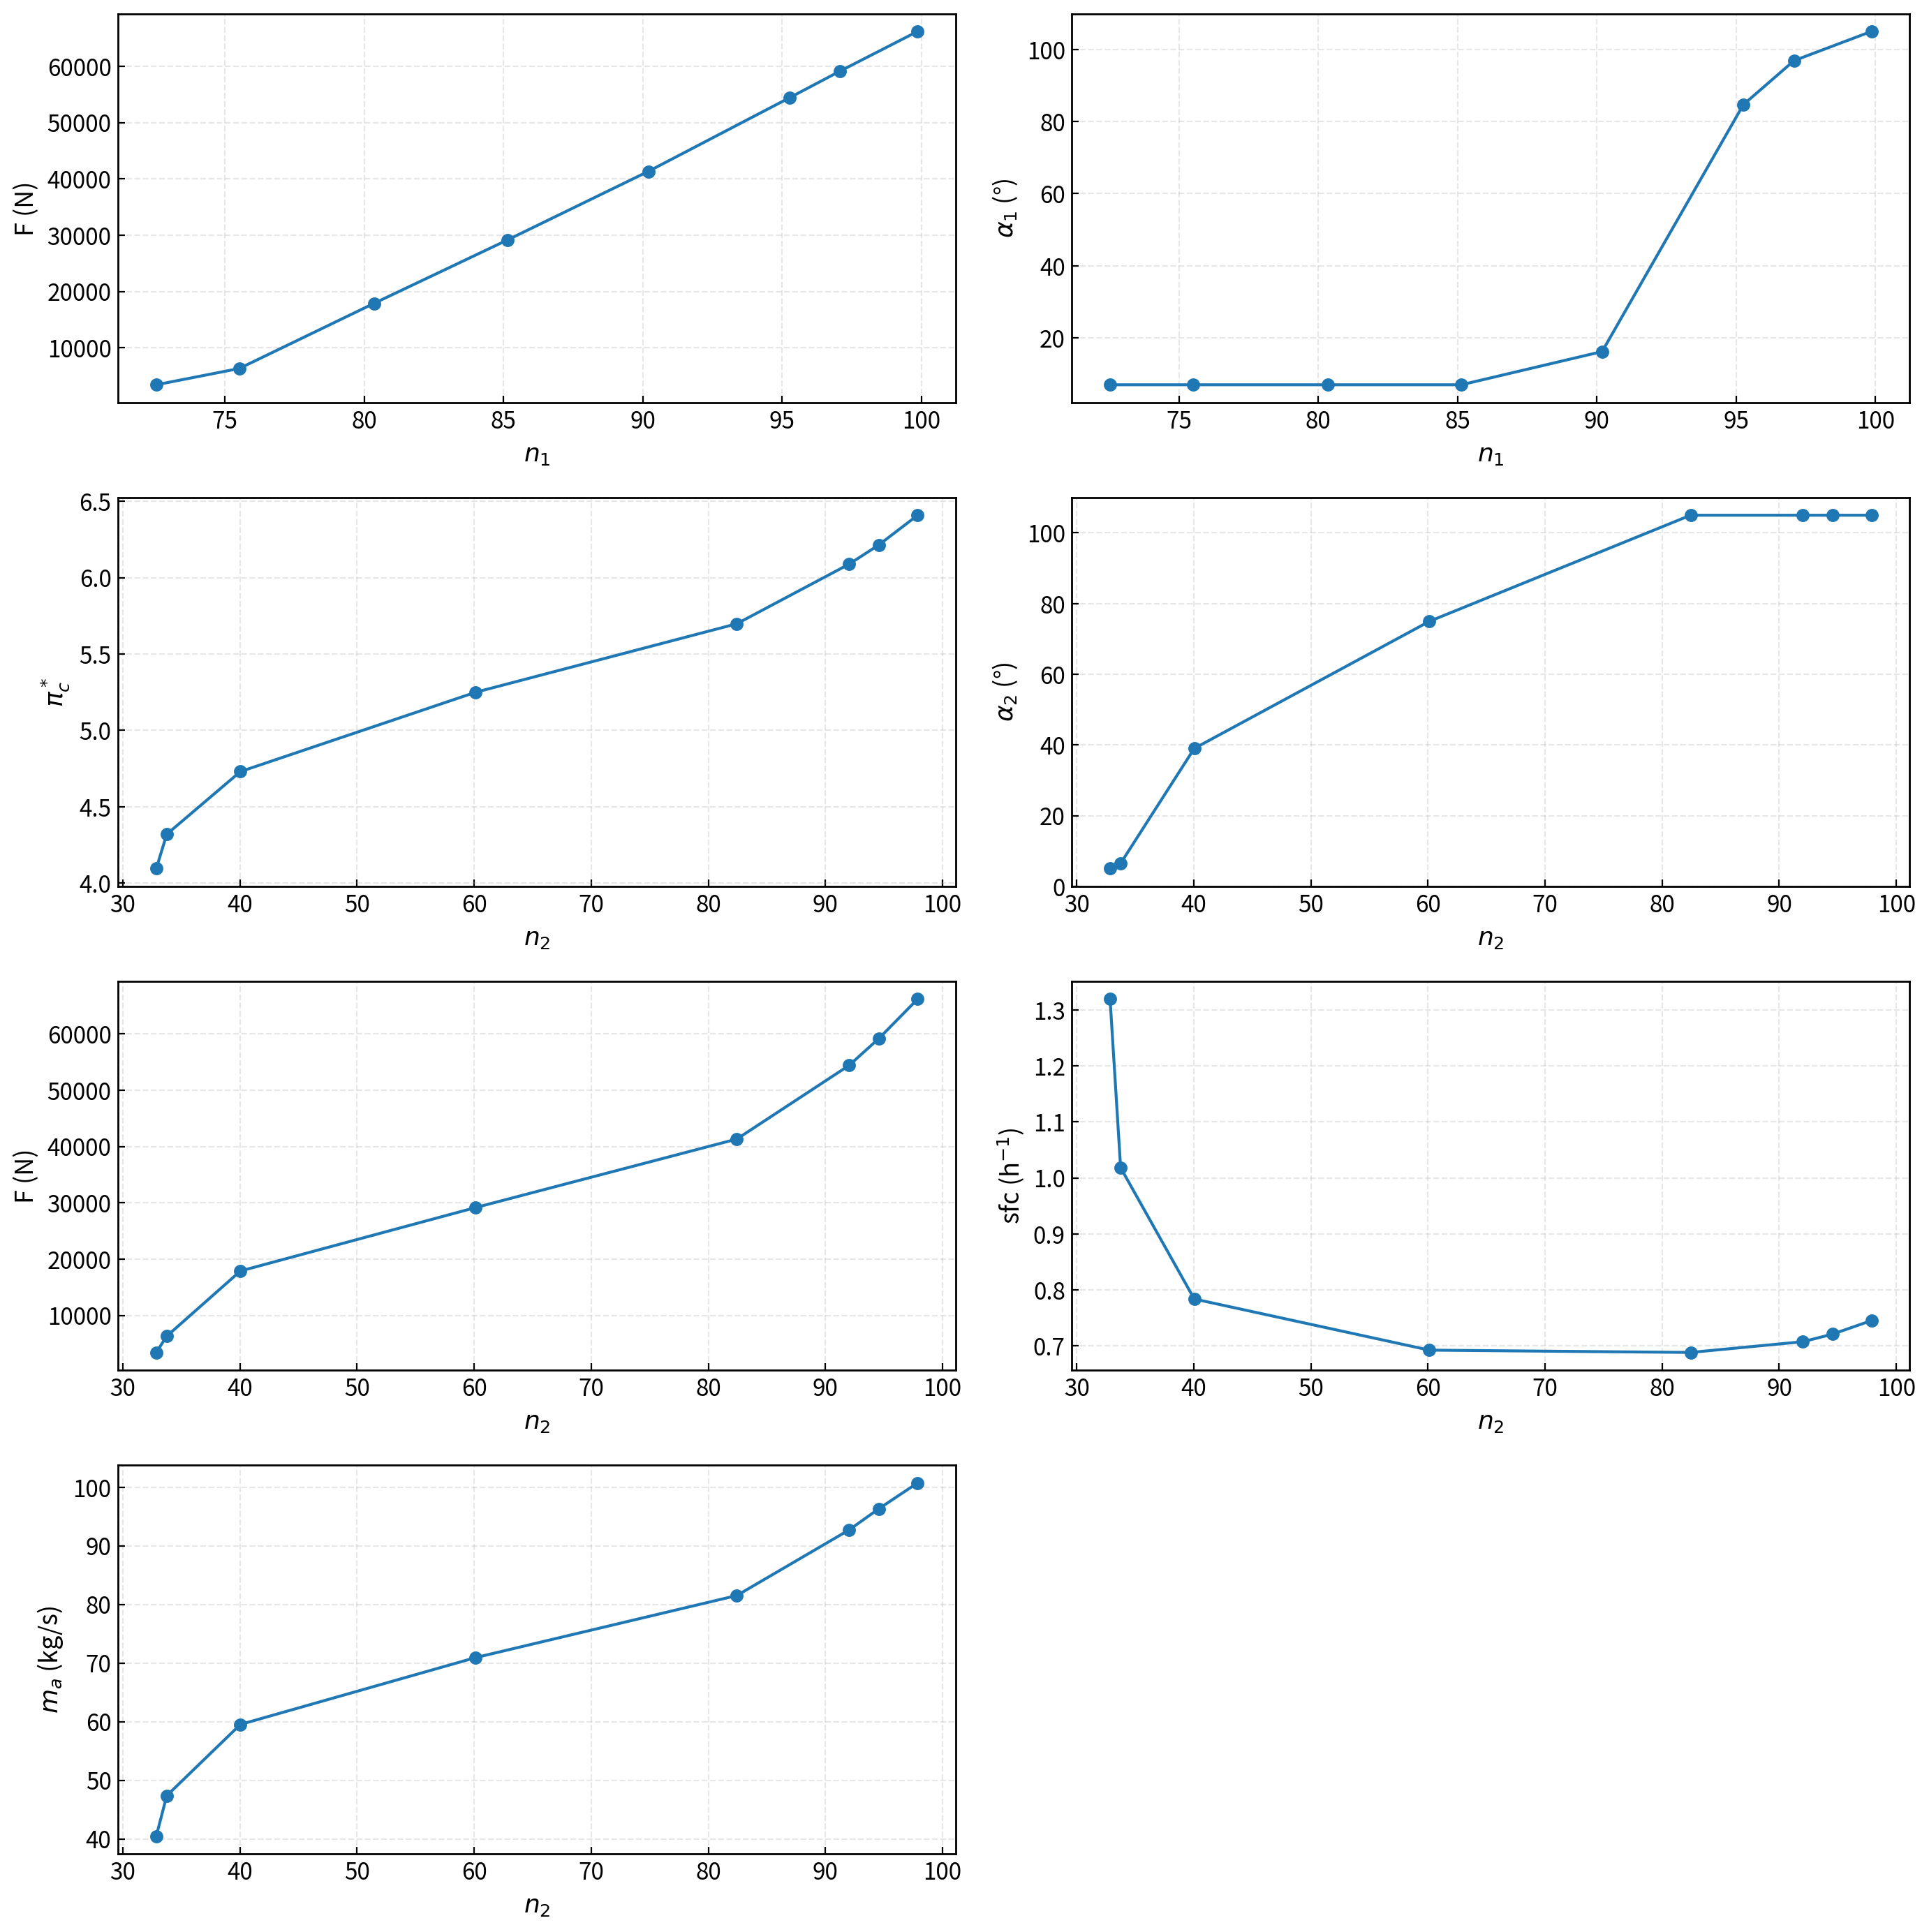
\includegraphics[width=\textwidth]{figures/exp1_throttle_characteristics.png}
    \caption{发动机节流特性曲线}
    \label{fig:throttle}
\end{figure}

\subsubsection{加力特性曲线}

\begin{figure}[H]
    \centering
    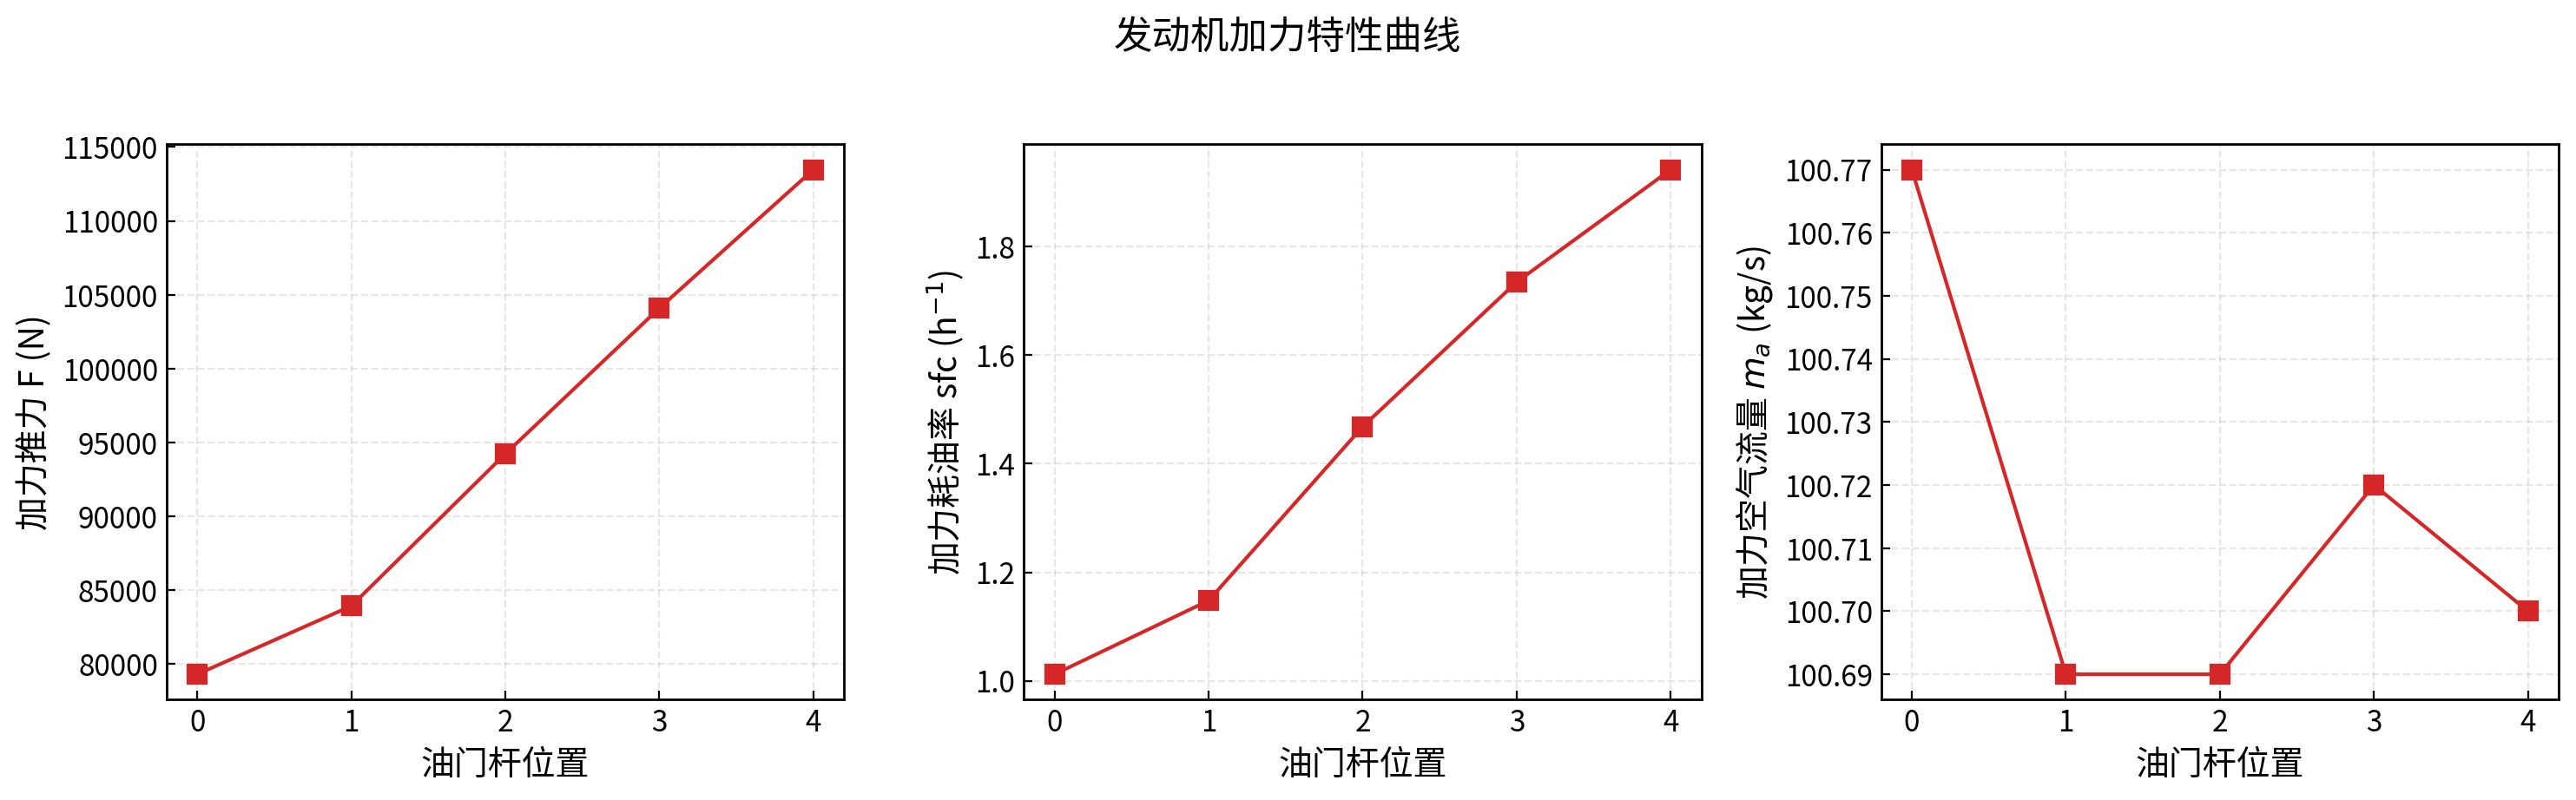
\includegraphics[width=\textwidth]{figures/exp1_afterburner_characteristics.png}
    \caption{发动机加力特性曲线}
    \label{fig:afterburner}
\end{figure}

\subsubsection{节流特性分析}

节流特性曲线（图~\ref{fig:throttle}）展示了发动机从慢车状态（$n_1=33\%, n_2=73\%$）到最大状态（$n_1=98\%, n_2=100\%$）各性能参数的变化规律。

\begin{enumerate}
    \item \textbf{推力特性}：推力 $F$ 随低压转速 $n_1$ 和高压转速 $n_2$ 均呈非线性快速增长。从慢车的 3.4 kN 增至最大状态的 66.2 kN，增幅约 19 倍。这是因为涡扇发动机推力近似与转速的三次方成正比，高转速下空气流量和单位推力同时增大。
    \item \textbf{耗油率特性}：sfc 从慢车的 1.32 h$^{-1}$ 降至 N2=90\% 时的 0.69 h$^{-1}$（最低点），随后在最大状态回升至 0.75 h$^{-1}$。sfc 在中等转速区域存在最优值，低转速下因部件效率低导致 sfc 偏高，高转速下因燃烧室油气比增大也使 sfc 有所回升。
    \item \textbf{增压特性}：压气机总压比 $\pi_c^*$ 随转速单调增加，从慢车的 4.09 升至最大状态的 6.41，反映了压气机增压能力随转速增大而增强。
    \item \textbf{空气流量}：$m_a$ 从 40.4 kg/s 增至 100.7 kg/s，与高压转速近似线性相关。
    \item \textbf{导叶调节}：进口导流叶片角度 $\alpha_1$ 从慢车时的 7° 增大至最大状态的 105°，$\alpha_2$ 从 5° 增至 105°，以保持各级攻角在合理范围。
\end{enumerate}

\subsubsection{加力特性分析}

加力特性曲线（图~\ref{fig:afterburner}）展示了从最小加力（$a_0=83$）到最大加力（$a_0=115$）五个加力状态的变化。

\begin{enumerate}
    \item \textbf{推力增幅}：加力推力从 79.3 kN 增至 113.5 kN，增幅约 43\%。相比最大非加力状态（66.2 kN），加力推力最多可提升约 71\%。
    \item \textbf{耗油率恶化}：加力 sfc 从 1.01 h$^{-1}$ 升至 1.94 h$^{-1}$，恶化约 92\%。加力状态下大量燃油在涡轮后喷入加力燃烧室，燃烧效率低于主燃烧室，导致耗油率急剧增大。
    \item \textbf{空气流量}：加力状态下 $m_a$ 基本维持在 100.7 kg/s，与最大非加力状态相同，表明加力主要通过增加燃油量（$W_f$ 从 5027 增至 22462 kg/h）而非增加空气流量来实现推力增推。
\end{enumerate}


\subsection{结论}

通过发动机模拟试车实验，获得了节流状态和加力状态下发动机主要性能参数的变化规律。实验数据表明：推力随转速非线性增大，sfc 在 N2=90\% 附近存在最优值，$\pi_c^*$ 和 $m_a$ 随转速单调增加。加力状态下推力可提升约 71\%，但 sfc 恶化约 92\%，体现了推力与耗油率之间的矛盾关系。实验结果符合涡扇发动机热力循环的基本原理。
